
\chapter{自动化检测工具}\label{chapter_system}

本章将介绍安卓控件启动的流程,及检测内存泄露的原理。

\section{安卓服务}
安卓应用中的服务可以通过两种方式启动\cite{service}:

\textbf{start 方式 } 其他组件构造特定的\textbf{Intent}对象,通过调用\textbf{startService() API}来启动目标服务。

\textbf{bind 方式 } 通过调用\textbf{bindService() API}将目标服务与特定组件绑定。被绑定的服务提供接口供其他组件与之交互。
一个服务可以同时通过以上两种方式启动。

\subsection{服务的生命周期}
服务的生命周期根据启动方式不同分为两种\cite{service}:

\textbf{start 方式 } 通过\textbf{startService() API}启动的服务将会一直运行,直到调用\textbf{stopSelf()}方法将自己停止运行。其他组件也可以通过调用\textbf{stopService() API}将服务停止运行。

停止运行的服务将会被\textbf{GC(Garbage Collector)}回收。

\textbf{bind 方式 } 通过\textbf{bindService() API}启动的服务将通过\textbf{IBinder}接口与其他组件进行交互,直到其他组件调用\textbf{unbindService() API}解除绑定。

一个服务可以同时绑定到多个组件之上,直到所有组件都解除了绑定时,该服务才会被\textbf{GC}回收。

每个安卓应用都关联一个\textbf{ActivityThread}实例,负责调度和执行该应用的各种组件。\textbf{ActivityThread}有一个\textbf{ArrayMap}类型的成员变量\textbf{mServices},其中保存了所有没有被销毁的服务的引用。一旦某个服务的实例被销毁,其引用将会从\textbf{mServices}中删除。

\subsection{服务的注册方式}
\begin{listing}[htbp]
	\centering
	\caption{服务的注册方式}
	\begin{minted}[encoding=utf8,
	frame=single,
	framesep = 1em,
	numbers=left, 
	breaklines=true, 
	tabsize=4,
	xleftmargin=2em,xrightmargin=2em,
	fontsize=\footnotesize]{xml}
<manifest
    xmlns:android="http://schemas.android.com/apk/res/android"
    xmlns:dist="http://schemas.android.com/apk/distribution"
    package="com.example.myapplication">
    <dist:module dist:instant="true" />
    <application ...>
        ...
        <service android:name=".Service1"
            android:enabled="true"
            android:exported="true">
        </service>
        <service
            android:name = ".Service2"
            android:enabled = "true"
            android:exported = "false">
            <intent-filter>
                <category android:name = "cat1"/>
                <action android:name = "act2"/>
            </intent-filter>
        </service>
        <service android:name = ".Service3"
            android:enabled = "true"
            android:permission = "Permission1">
            <intent-filter>
                <action android:name = "act3"/>
                <category android:name = "cat2"/>
                <data android:scheme = "Scheme1"/>
                <data android:scheme = "Scheme2"/>
            </intent-filter>
        </service>
    </application>
</manifest>
	\end{minted}
	\label{declaration:service}
\end{listing}
通常,每个服务都要在\textbf{AndroidManifest.xml}中注册一个\textbf{<service>}标签(参考Listing.\textcolor{red}{\ref{declaration:service}}中的样例)。同时服务可以通过设置"\textbf{android:exported}"属性来指定该服务是否将被导出。当设置\textbf{android:exported = "true"}时,该服务可以被其他应用使用,反之不可。
%可以凑更多字数
\subsection{服务的内存泄漏}\label{service_leak}
通常,一个服务的实例不再被使用时应该被\textbf{GC(Garbage Collector)}回收,并释放资源。然而在某些情况下,一个被销毁的服务可能会意外的被引用,从而使得\textbf{GC}无法将其回收并释放资源,这样就造成了服务的内存泄漏。
\begin{listing}[htbp]
	\centering
	\caption{服务的内存泄漏}
	\begin{minted}[encoding=utf8,
		frame=single,
		framesep = 1em,
		numbers=left, 
		breaklines=true, 
		tabsize=4,
		showtabs = false,
		xleftmargin=2em,xrightmargin=2em,
		fontsize=\footnotesize]{java}
public class LeakedService extends Service{
	private static final String TAG = "LeakedService";
	// Method will be called when an instance is creating.
	public void onCreate(){
		...
		new Timer().scheduleAtFixedRate(new TimerTask(){
			public void run(){
				Log.d(TAG, LeakedService.this.getPackageName() + ".LeakedService is running!");
			}
		},1000L,3000L);
	}
	// Method will be called when an instance is destroying.
	public void onDestroy(){
		...
	}
}
	\end{minted}
	\label{leaked example:service}
\end{listing}

例如在游戏\emph{com.siendas.games2048}中,就出现了原理如图(见\textbf{Listing.\textcolor{red}{\ref{leaked example:service}}})的内存泄漏。具体导致内存泄露的原理为:在\textbf{LeakedService}的实例被构造的时候,将会调用他的\textbf{onCreate()}方法,在该方法中延迟\textbf{1000ms}启动了一个\textbf{匿名}计时器,该计时器将以\textbf{3000ms}的周期打印调试信息,可以看到在\textbf{TimerTask}类中持有了\textbf{LeakedService}的引用,而在该服务被销毁时,其\textbf{onDestroy()}方法中并没有对该匿名计时器进行销毁。因此在该服务被销毁后,将会一直存在一个匿名计时器持有该服务的引用,导致\textbf{GC}无法将其回收,从而导致了内存泄漏。

\section{安卓广播接收器}
安卓应用中的广播接收器亦有两种方式启动\cite{broadcast}:

\textbf{清单声明的接收器 }\label{declaration:receiver in manifest} 通过在\textbf{AndroidManifest.xml}中添加\textbf{<receiver>}标签注册广播接收器,通过\textbf{<intent-filter>}标签指定接收器所订阅的广播操作。系统软件包管理器会在应用安装时注册接收器。然后,该接收器会成为应用的一个独立入口点,这意味着如果应用当前尚未运行,系统可以启动应用并发送广播。系统会创建新的\textbf{BroadcastReceiver}组件对象来处理它接收到的每个广播。次对象仅在调用\textbf{onReceive(Context, Intent)}期间有效。一旦从此方法返回代码,系统便会认为该组件不再活跃。

\textbf{上下文注册的接收器 }\label{declaration:receiver in context} 通过在代码中构造出\textbf{BroadReceiver}实例,以及\textbf{IntentFilter}实例来指定订阅的广播内容,调用\textbf{registerReceiver(BroadcastReceiver, IntentFilter) API}来注册接收器。只要上下文有效,通过改种方式注册的广播接收器就会接收广播。如果要停止接收广播,需要调用\textbf{unregisterReceiver(BroadcastReceiver) API}来注销广播接收器

\subsection{广播接收器的生命周期}
广播接收器的生命周期根据启动方式不同亦分为两种\cite{broadcast}:

\textbf{清单声明的接收器 } 静态注册的接收器生命周期不限于\textbf{Activity}甚至整个应用。即使应用并不在运行,接收器也可以接收到订阅的广播。将会在\textbf{onReceive()}方法结束后被销毁。


\textbf{上下文注册的接收器 } 上下文注册的接收器,其生命周期仅限于注册的上下文,例如在\textbf{Activity}上下文注册的接收器,在整个\textbf{Activity}存活期间可以持续接收广播;在应用上下文中注册的接收器,则会在整个应用运行期间都可以接收广播。需要注意的是:这种方式启动的接收器必须手动进行销毁,即调用\textbf{unregisterReceiver() API},否则在上下文失效时,系统会抛出异常(并不会导致应用崩溃),同时接收器会引发泄露(见图.\textcolor{red}{\ref{fig:broadcast_leak}})。

\begin{figure}[htbp]
   \centering
   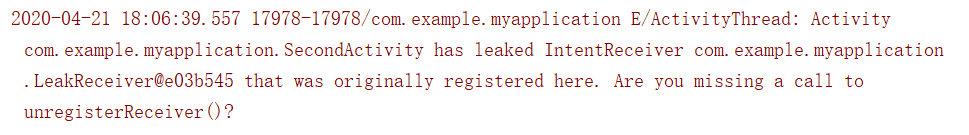
\includegraphics[width=0.9\textwidth]{broadcast_leak.png} % requires the graphicx package
   \caption{没有回收接收器将会导致异常以及泄露}
   \label{fig:broadcast_leak}
\end{figure}

\subsection{广播接收器的注册方式}
\begin{listing}[htbp]
	\centering
	\caption{广播接收器的注册方式}
	\begin{minted}[encoding=utf8,
	frame=single,
	framesep = 1em,
	numbers=left, 
	breaklines=true, 
	tabsize=4,
	showtabs = false,
	xleftmargin=2em,xrightmargin=2em,
	fontsize=\footnotesize]{XML}
<manifest 
	xmlns:android="http://schemas.android.com/apk/res/android"
	xmlns:dist="http://schemas.android.com/apk/distribution"
	package="com.example.myapplication">
	<dist:module dist:instant="true" />
	<application ...>
		...
		<receiver
			android:name = ".Receiver1">
			<intent-filter>
				<action android:name = "act1" />
			</intent-filter>
		</receiver>
		<receiver
			android:name = ".Receiver2"
			android:exported = "false"
			android:enabled = "true">
			<intent-filter>
				<category android:name = "cat1" />
				<action android:name = "act2" />
			</intent-filter>
		</receiver>
	</application>
</manifest>
	\end{minted}
	\label{declaration:receiver}
\end{listing}

一般而言,清单声明的广播接收器(见\ref{declaration:receiver in manifest})需要在\textbf{AndroidManifest.xml}文件中添加\textbf{<receiver>}标签(参考\textbf{Listing.\textcolor{red}{\ref{declaration:receiver}}}),在\textbf{<intent-filter>}子标签中可以指定订阅的广播内容等,也可以通过设置\textbf{"android:exported"}属性来指定该广播是否将被导出。而上下文注册的广播接收器(见\ref{declaration:receiver in context})则不需要进行前文的操作。
\subsection{广播接收器的内存泄漏}
广播接收器的内存泄漏原理类似与服务内存泄漏\ref{service_leak}。但是由广播接收器引起的内存泄漏往往比服务更为严重,因为广播接收器被系统认为只进行不耗时的操作(如果超过10s未从\textbf{onReceive()}方法中返回,将抛出\textbf{ANR Exception}),因此通常广播接收器在接到广播后,很有可能会启动其他的\textbf{Service}进行后续的耗时操作,进而可能会导致一连串的内存泄漏。

例如图中(见\textbf{Listing.\textcolor{red}{\ref{leaked example:receiver}}})所示的广播接收器,不仅本身会导致内存泄漏,而且还会启动一个会导致内存泄漏的服务(见\textbf{Listing.\textcolor{red}{\ref{leaked example:service}}}),因此后果将会更加严重。
\begin{listing}[htbp]
	\centering
	\caption{广播接收器的内存泄漏}
	\begin{minted}[encoding=utf8,
	frame=single,
	framesep = 1em,
	numbers=left, 
	breaklines=true, 
	tabsize=4,
	showtabs = false,
	xleftmargin=2em,xrightmargin=2em,
	fontsize=\footnotesize]{java}
public class LeakReceiver extends BroadcastReceiver {
	private final String TAG = "LeakReceiver";
	private final int ID = new Random().nextInt();
	@Override
	public void onReceive(Context context, Intent intent) {
		...
		context.startService(new Intent(context,LeakService.class));
		new Timer().scheduleAtFixedRate(new TimerTask() {
			@Override
			public void run() {
				Log.i(TAG,LeakReceiver.this.ID + " is running!");
			}
		}, 1000L, 3000L);
	}
}
	\end{minted}
	\label{leaked example:receiver}
\end{listing}
\section{自动化检测工具原理}
\begin{figure}[htbp]
	\centering
	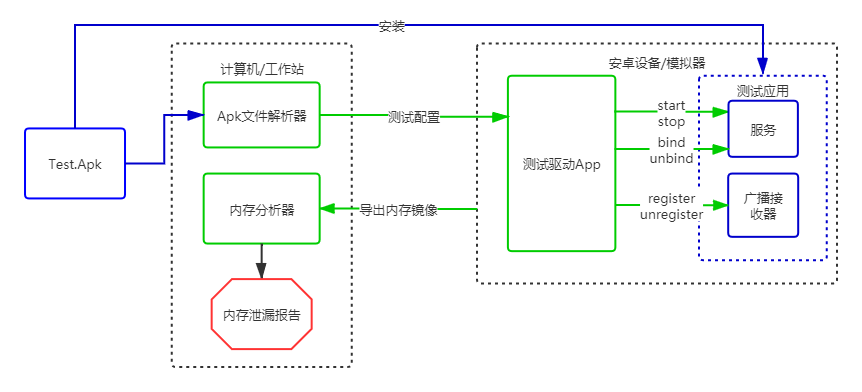
\includegraphics[width=0.9\textwidth]{main_flow.png} % requires the graphicx package
	\caption{自动检测工具原理}
	\label{fig:flow}
\end{figure}

如图\textbf{\textcolor{red}{\ref{fig:flow}}}所示,测试将在两个环境(工作站、安卓模拟器)中完成:
\begin{enumerate}
	\item 在工作站中,使用\textbf{Apk文件解析器}(详见\textbf{\textcolor{red}{\ref{apk analyser}}})对被测试应用\textbf{Test.apk}进行反编译,并解析\textbf{AndroidManifest.xml}清单,得到在清单中注册的\textbf{公开服务}以及\textbf{清单声明的广播接收器},作为测试对象生成一份\textbf{测试配置}发送到安卓模拟器上。
	\item 在安卓模拟器上安装好\textbf{测试驱动App}(详见\redbf{\ref{test driver app}})以及被测试应用\textbf{Test.apk}。通过\textbf{ADB}向安卓模拟器发送指令启动\textbf{测试驱动App},它会读取步骤1中发送来的\textbf{测试配置},然后执行测试主流程(详见\redbf{\ref{main flow}})
	\item 在完成测试主流程之后,通知工作站将被测试应用的堆镜像文件(.prof)文件导出,使用\textbf{内存分析器}(详见\redbf{\ref{memory analyser}})进行内存泄漏的检测,最终生成一份\textbf{内存泄漏报告}显示被测试应用的服务以及广播接收器有无内存泄漏情况,以及具体的内存泄漏的控件清单。
\end{enumerate}

\subsection{Apk 文件解析器}\label{apk analyser}
Apk 文件解析器旨在通过将被测试应用反编译得到\textbf{AndroidManifest.xml}清单,对该清单进行分析,从而得到在清单中声明的\textbf{公开服务}以及\textbf{广播接收器}作为测试对象。
\begin{listing}[htbp]
	\centering
	\caption{使用apktool工具进行apk的反编译}
	\begin{minted}[encoding=utf8,
	frame=single,
	framesep = 1em,
	numbers=left, 
	breaklines=true, 
	tabsize=4,
	showtabs = false,
	xleftmargin=2em,xrightmargin=2em,
	fontsize=\footnotesize]{shell}
apktool d -f $test_apk$ -o temp
	\end{minted}
	\label{shell:apktool}
\end{listing}

使用apktool工具\cite{apktool},执行\textbf{Listing.}\redbf{\ref{shell:apktool}}中的命令即可完成被测试应用的反编译得到\textbf{AndroidManifest.xml}清单。

\begin{listing}[htbp]
	\centering
	\caption{使用python解析xml输出测试配置}
	\begin{minted}[encoding=utf8,
	frame=single,
	framesep = 1em,
	numbers=left, 
	breaklines=true, 
	tabsize=4,
	showtabs = false,
	xleftmargin=2em,xrightmargin=2em,
	fontsize=\footnotesize]{python}
from xml.dom.minidom import parse
def get_exported_services(xml_path):
	exported_services = []
	manifest = parse(xml_path).documentElement 
	for service in manifest.getElementsByTagName('service'):
		exported = service.getAttribute('android:exported')
		enabled = service.getAttribute('android:enabled')
		if (exported == 'true' and (enabled == '' or enabled == 'true')):
			exported_services.append(service)
	return exported_services
	
def get_static_receivers(xml_path):
	exported_receivers = []
	domTree = parse(xml_path)
	manifest = domTree.documentElement
	for receiver in manifest.getElementsByTagName('receiver'):
		enabled = receiver.getAttribute('android:enabled')
		if (enabled == '' or enabled == 'true'):
			exported_receivers.append(receiver)
	return exported_receivers;
	\end{minted}
	\label{python:get services}	
\end{listing}

接下来使用\textbf{python}中的\textbf{xml} 库解析此xml文件(详见\textbf{Listing.}\redbf{\ref{python:get services}}),筛选出所有指定\textbf{android:exported = "true"} 以及 \textbf{android:enabled = "true"}(或者不指定,默认值为"true")的服务,以及在清单中声明的广播接收器。将这些控件的包名,类名,以及所需的权限等信息写入\textbf{测试配置}中
\subsection{测试驱动App}\label{test driver app}
测试驱动App负责控制所有安卓模拟器上的测试行为(即测试主流程\redbf{\ref{main flow}})。首先驱动会读取\textbf{测试配置},获得要测试的服务和广播接收器,之后进行\textbf{测试主流程},在完成测试流程之后,使用\textbf{Socket}与\textbf{工作站}进行通信,通知\textbf{工作站}测试任务已经完成,导出被测试应用的堆镜像文件进行最后的分析。
\subsection{测试主流程}\label{main flow}

\begin{algorithm}
	\caption{测试主流程:公开服务测试}
	\label{alg:service}
	\begin{algorithmic}[1]
		\STATE {读取测试配置}
		\FOR{遍历测试配置中的公开服务}
			\STATE{重置安卓模拟器}
			\STATE{重置计数器}
			\IF{使用bind方式测试}
				\STATE{启动仿真Activity}
			\ENDIF
			\WHILE{计时器 < 测试重复次数}
				\IF{使用start方式测试}
					\STATE {调用startService() API 启动服务} 
					\STATE {调用stopService() API 停止服务}
				\ELSE
					\STATE{调用bindService() API 将服务绑定到Activity上}
					\STATE{调用unbindService() API 解除服务绑定}
				\ENDIF
				\STATE{计数器自增1}
			\ENDWHILE
			\IF{使用bind方式测试}
				\STATE{销毁仿真Activity}
			\ENDIF
			\STATE{通知工作站导出堆镜像}
		\ENDFOR
	\end{algorithmic}
\end{algorithm}

\begin{algorithm}
	\caption{测试主流程:清单声明的广播接收器}
	\label{alg:receiver}
	\begin{algorithmic}[1]
		\STATE {读取测试配置}
		\FOR{遍历测试配置中的广播接收器}
			\STATE{重置安卓模拟器}
			\STATE{重置计数器}
			\WHILE{计时器 < 测试重复次数}
				\STATE{构造特定广播,定向发送给该接收器}
				\STATE{计数器自增1}
			\ENDWHILE
			\STATE{通知工作站导出堆镜像}
		\ENDFOR
	\end{algorithmic}
\end{algorithm}

在测试主流程中,对服务和接收器进行逐一测试:

\textbf{服务测试(见算法\redbf{\ref{alg:service}}) }  测试原理为对被测试应用进行大量重复的启动和关闭(根据测试要求不同分为start/bind 和stop/unbind),确保潜在的内存泄漏被触发,之后将被测试应用的堆镜像导出,送入\textbf{内存分析器}(详见\redbf{\ref{memory analyser}})进行检测和分析。

\textbf{广播接收器测试(见算法\redbf{\ref{alg:receiver}}) }
广播接收器的测试不需要事先启动应用,因为在清单中注册的广播接收器在应用安装时就会在系统中进行注册,在任何时候都可以接收广播(即使应用未运行),因此只需要构造接收器订阅的广播,定向发送给该接收器就可以触发该接收器。同样的为了确保潜在的内存泄漏被触发,需要重复发送大量的广播。最终将被测试应用的堆镜像导出,送入\textbf{内存分析器}(详见\redbf{\ref{memory analyser}})进行检测和分析。
\subsection{内存分析器}\label{memory analyser}

\begin{algorithm}
	\caption{内存分析器:服务分析}
	\label{alg:memory analyser:service}
	\begin{algorithmic}[1]
		\STATE{导入并解析.hprof文件}
		\STATE{查询所有Service的衍生类集合}
		\FOR {遍历Service的衍生类集合}
			\IF{该实例已经被销毁}
				\STATE{获得所有该实例到GC Root的路径集合}
				\STATE{去除路径集合中不合理的路径}
				\IF[证明该实例确实已经被销毁]{路径集合为空}
					\STATE{该实例不存在内存泄漏}
				\ELSE[该实例仍然被引用,产生内存泄漏]
					\STATE{该实例产生内存泄漏}
					\IF{该实例内存泄漏原因为已知的安卓系统BUG}
						\STATE{不判定构成人为内存泄漏}
					\ELSE
						\STATE{由开发者构成的人为内存泄漏}
					\ENDIF
				\ENDIF
			\ENDIF
		\ENDFOR
	\end{algorithmic}
\end{algorithm}

\begin{algorithm}
	\caption{内存分析器:服务分析}
	\label{alg:memory analyser:receiver}
	\begin{algorithmic}[1]
		\STATE{导入并解析.hprof文件}
		\STATE{查询所有BroadcastReciver的衍生类集合}
		\FOR {遍历BroadcastReceiver的衍生类集合}
			\IF{该实例已经被销毁}
				\STATE{获得所有该实例到GC Root的路径集合}
				\STATE{去除路径集合中不合理的路径}
				\IF[证明该实例确实已经被销毁]{路径集合为空}
					\STATE{该实例不存在内存泄漏}
				\ELSE[该实例仍然被引用,产生内存泄漏]
					\STATE{该实例产生内存泄漏}
					\IF{该实例内存泄漏原因为已知的安卓系统BUG}
						\STATE{不判定构成人为内存泄漏}
					\ELSE
						\STATE{由开发者构成的人为内存泄漏}
					\ENDIF
				\ENDIF
			\ENDIF
		\ENDFOR
	\end{algorithmic}
\end{algorithm}

内存分析器负责从堆镜像文件(\textbf{.hprof文件})中识别和统计服务(广播接收器)的内存泄漏实例,基于开源工具MAT\cite{mat}进行定制化的开发,具体原理(详见\textbf{算法\redbf{\ref{alg:memory analyser:service}}及\redbf{\ref{alg:memory analyser:receiver}}})为:首先导入并解析堆镜像文件,找到所有的服务(广播接收器)实例,接下来对于每个找到的实例,逐个检测判断是否产生了内存泄露,对于产生内存泄漏的控件,生成一份内存泄漏分析报告。

\textbf{服务的内存泄露判定 } 所有仍然活跃的服务都会被\textbf{ActivityThread} 的 \textbf{mServices}变量所引用,而所有被销毁的服务都会被从\textbf{mServices}中删除。一个对象的实例如果实际上处于存活状态,则一定会拥有至少一条有效的\textbf{GC Root Path}。因此服务内存泄漏的判定充要条件为:拥有至少一条有效的\textbf{GC Root Path}且不在\textbf{mServices}中。

\textbf{广播接收器的内存泄漏判定 } 由于广播接收器被系统规定为不耗时控件(超过10s未完成\textbf{onReceive()} 方法,将会抛出\textbf{ANR Exception}导致应用崩溃),因此对于广播接收器而言,只需要检测是否有实际处于存活状态的实例即可。即:拥有至少一条有效的\textbf{GC Root Path}。

\textbf{安卓系统自身原因产生内存泄漏 } 由于安卓系统自身可能存在\textbf{BUG}导致正常的控件产生内存泄漏,此类问题并非由于安卓应用开发者的失误而导致,因此要将此类内存泄漏排除。

\subsection{实现细节}

\textbf{后台服务限制 }\cite{android-service-limit} 在安卓8中,新增了“电池优化策略”,系统不允许后台应用创建后台服务,因此跨应用对服务进行测试将会失败。解决办法为:禁用系统的电池管理服务;在测试时,将被测试应用置于前台。

\textbf{广播限制 }\cite{android-receiver-limit} 在\textbf{安卓8}及更高版本系统的应用中禁止将隐式广播注册为清单声明的广播接收器。而显示广播和需要签名授权的广播接收器不受限制,可以继续注册为清单声明的广播接收器。\textbf{注意:}随着安卓系统的更新,很多隐式广播已经不再受到此规定的限制,具体的广播列表可以参考隐式广播例外\cite{android-receiver-limit-exception}。

\textbf{超级用户限制 } 在\textbf{安卓7}以及更早的版本中,开发者经常会将系统增加超级用户权限,以便于进行测试(亦成为\textbf{root}),大致的方法为将兼容的二进制文件\textbf{su}拷贝到安卓设备中,使安卓设备可以执行超级用户指令\textbf{sudo},进而为测试带来便利。然而再\textbf{安卓8}以及更高的系统中,由于用于\textbf{root}操作的二进制文件\textbf{su}维护团队相继解散,获得非安卓系统开发人员获得超级用户权限变得困难,因此本文的自动化检测工具的实现不要求对系统进行\textbf{root},而将使用\textbf{socket}建立安卓设备与工作站的通信,由工作站使用\textbf{adb}指令完成跨应用的特殊权限操作:比如\textbf{跨应用导出堆镜像文件}操作需要应用拥有超级用户权限,而使用\textbf{adb}指令则不需要超级用户权限即可导出任意应用的堆镜像文件。